    \cleardoublepage
\section*{Avant-propos
    \label{body:avant-propos}
    }
    \addcontentsline{toc}{part}{Avant-propos}
    \markboth{Avant-propos}{}
    \markright{Préambule}{}

    % Figure logo HdF
\begin{wrapfigure}[6]{r}{0.2\textwidth} % 6 lignes pour ajuster la hauteur
    \vspace{-10pt} % Réduit l'espacement vertical avant la figure
    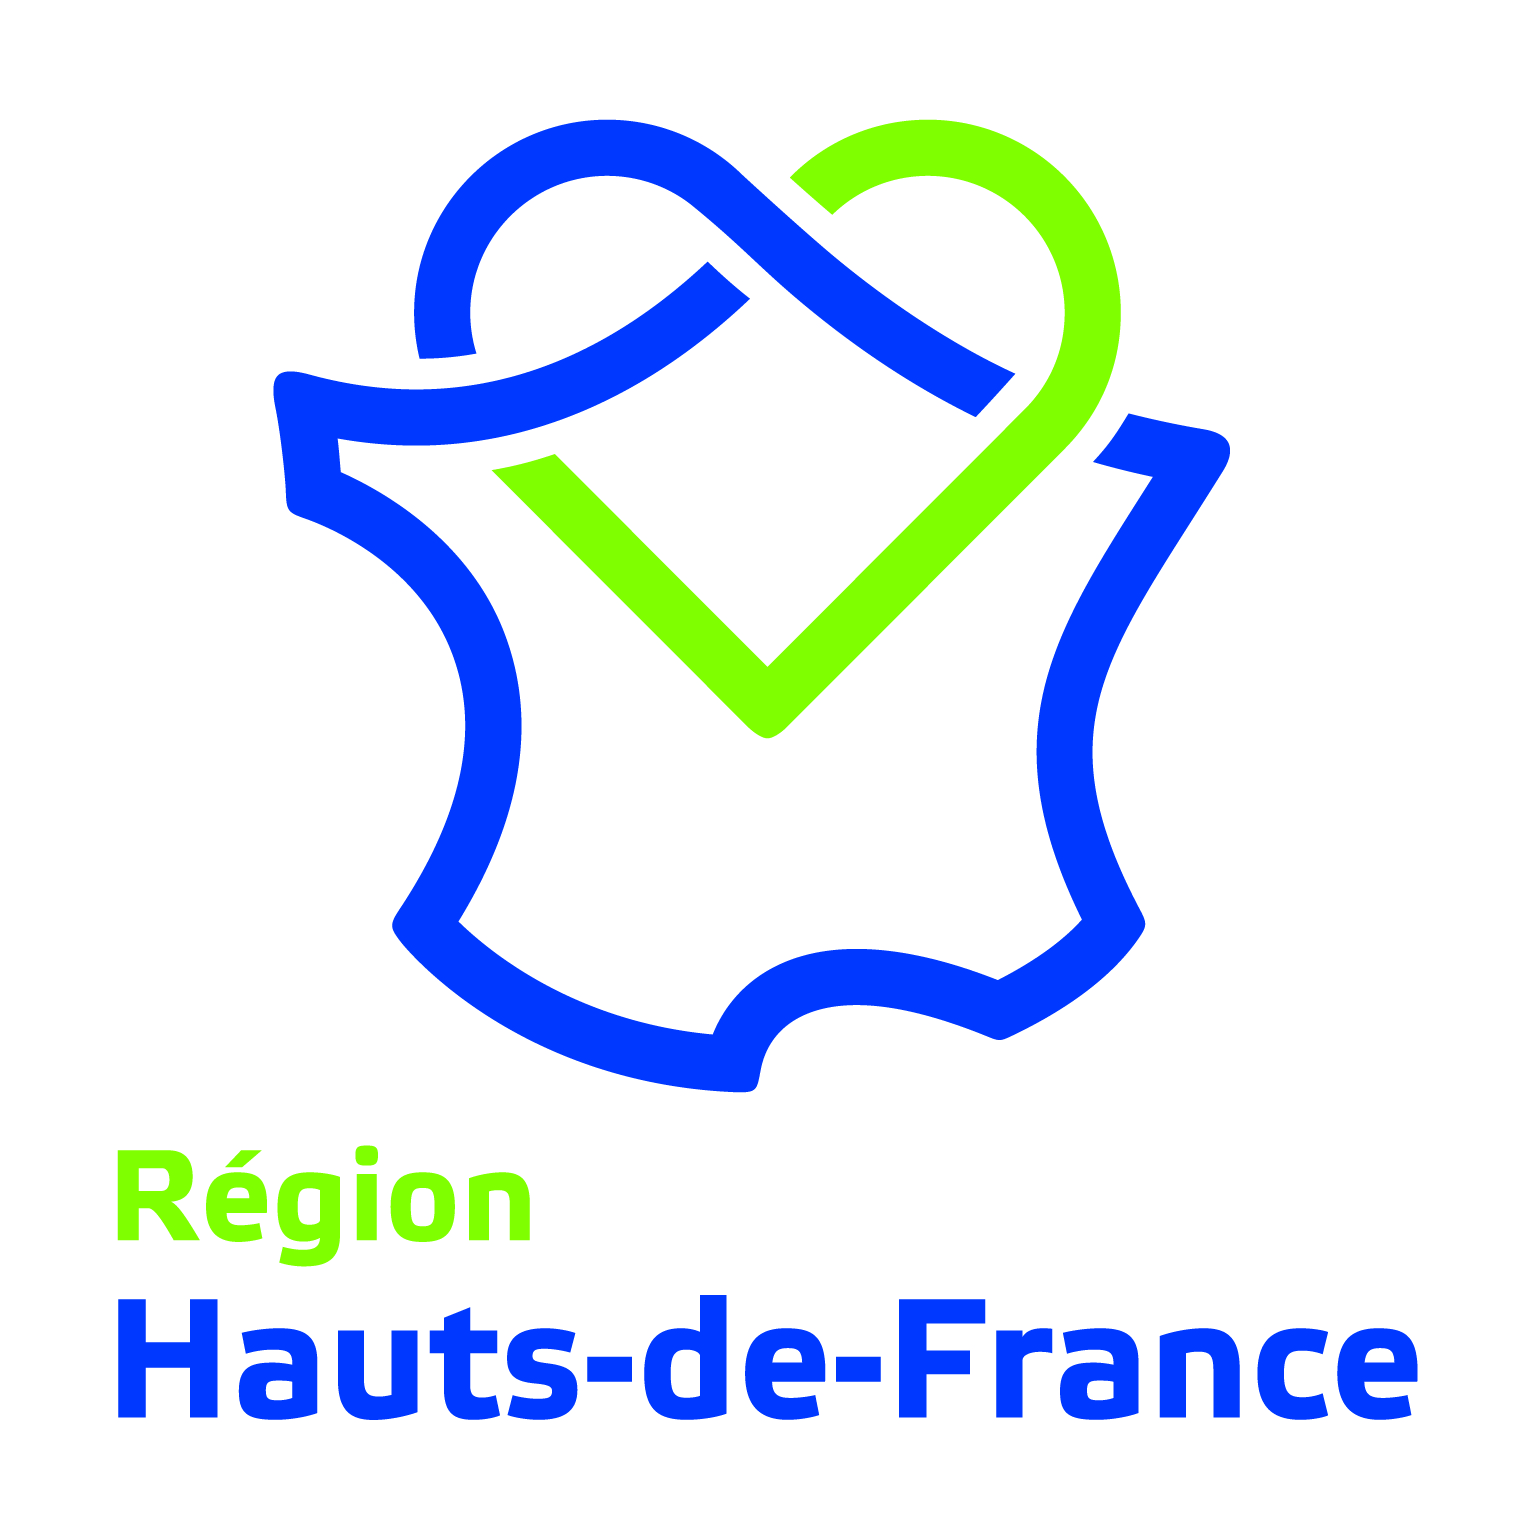
\includegraphics[width=\linewidth]{src/Figures/Introduction/Logo_HdF.jpg} 
    \caption*{}
    \label{fig-introduction:logo-hdf}
\end{wrapfigure}

    % Introduction
Cette recherche doctorale a été menée à l'Université Gustave Eiffel\footnote{
    L’Université Gustave Eiffel est un \acrfull{EPSCP}, fondé en 2020 \textcolor{blue}{\autocite{universite_gustave_eiffel_notre_2024}}\index{Université Gustave Eiffel@\textsl{Université Gustave Eiffel}|pagebf}. Elle est issue de la fusion et du regroupement d’une université, d’un organisme de recherche et de plusieurs écoles, incluant notamment l’\acrfull{IFSTTAR}, l’\acrfull{UPEM} ainsi que d’autres établissements associés.
}, au sein du \acrfull{LVMT}\footnote{
    Le \acrfull{LVMT} est une \acrfull{UMR} fondée en 2003, placée sous la co-tutelle de l’Université Gustave Eiffel et de l’Institut Polytechnique de Paris, ce dernier étant issu d’un regroupement intégrant notamment l’\acrfull{ENPC}. Le \acrshort{LVMT} se consacre à l’étude des interactions entre les territoires, les transports et les mobilités, en mobilisant des approches pluridisciplinaires issues de l’aménagement, de l’urbanisme, de la géographie, de l’économie, de la sociologie, de l’anthropologie et des sciences de l’ingénieur \textcolor{blue}{\autocite{laboratoire_ville_mobilite_transport_presentation_2024}}\index{Laboratoire Ville Mobilité Transport@\textsl{Laboratoire Ville Mobilité Transport}|pagebf}.
}. Le contrat doctoral a été cofinancé par la Région Hauts-de-France, dans le cadre de l'initiative \textsl{rev3} (\textsl{Troisième Révolution Industrielle})\footnote{
    L’initiative \textsl{rev3} (\textsl{Troisième Révolution Industrielle}) est une dynamique collective lancée en 2013, copilotée par la Région Hauts-de-France et la \acrfull{CCI} Hauts-de-France. Elle vise à concevoir et à promouvoir des modèles innovants de développement des territoires, inscrits dans une perspective durable à l’horizon 2050 \textcolor{blue}{\autocite{rev3_rev3_2022}}\index{rev3@\textsl{rev3}|pagebf}.
}. Cette thèse de doctorat s'inscrit à la fois dans le deuxième \acrfull{COP} 2023-2025 de l'Université Gustave Eiffel\footnote{
    Elle s'inscrit plus particulièrement dans le Projet stratégique 2.1 (\Guillemets{Développer une mobilité décarbonée pour tous les usagers et sur tous les territoires en toute sécurité, en s’appuyant sur la compréhension des comportements et usages de mobilité}) et 2.4 (\Guillemets{Progresser dans les modèles de développement intégrant les Objectifs de développement durable}).
} et dans le troisième axe de recherche \Guillemets{Aménagement urbain et territoires}\footnote{
    L’axe 3 \Guillemets{Aménagement urbain et territoires} du \acrfull{LVMT} se consacre à l’étude des interactions entre les territoires, le transport et les mobilités \textcolor{blue}{\autocite{laboratoire_ville_mobilite_transport_axe_2024}}\index{Laboratoire Ville Mobilité Transport@\textsl{Laboratoire Ville Mobilité Transport}|pagebf}. Il explore les dynamiques territoriales et leur modélisation, le maillage des réseaux de transport, les modèles d’aménagement, ainsi que les enjeux liés à la sobriété énergétique. Les travaux menés dans ce cadre s’articulent autour de deux niveaux principaux d’interaction. D’une part, ils s’intéressent aux nœuds de transport, en examinant les flux qu’ils polarisent, les aménagements qu’ils génèrent et leur rôle stratégique pour les acteurs publics et privés. D’autre part, ils analysent la manière dont les réseaux de transport contribuent à renforcer les liens entre les territoires, tout en influençant les formes urbaines et les relations au sein des systèmes urbains régionaux.
} du \acrshort{LVMT}.%%Rédigé%%